\resourceheading{4}{30-Second Student Video Memo}{Student voice, formative communication, SEL \& behavior-as-communication\par}{Students, teachers, families \& support teams}{Implemented EDU486 post-activity video memos and de-identified source transcripts}

\vspace{-0.5cm}
\toolsection{The Existing Camp Artifact}

PTR improves how adults interpret evidence; the 30-second memo changes who gets to author that evidence. During the Invisible Invaders camp, youth were invited after an activity to explain in their own words what they did, how they experienced it, what they learned or confirmed, and what they wanted to investigate next. The reviewed Field Friday source index preserves a 43-second post-activity memo in which a youth described the sand-sampling work as hands-on, said they liked it, distinguished new learning from something confirmed, and connected the activity to a larger exposure question \citep{campEvidence2026}. This is a communication support because the learner, not an adult behavior rating, authors the first account of the activity. It also supports social-emotional learning by giving students a routine for recognizing how an experience affected them, naming what helped or did not help, and communicating what they want next. Preferences, confusion, sensory responses, questions, and change requests can become visible before adults reduce them to engagement, compliance, or disruption. The memo gives the next teacher, family member, or collaborator evidence for redesign.

\toolsection{Four Prompts, One Student-Owned Record}

Use the memo after each major activity while keeping the time, mode, and decision to participate flexible.

\small
\renewcommand{\arraystretch}{1.00}
\setlength{\tabcolsep}{3pt}

\begin{tabularx}{\textwidth}{
>{\bfseries\RaggedRight\arraybackslash}p{0.90in}
>{\RaggedRight\arraybackslash}p{2.35in}
>{\RaggedRight\arraybackslash}X}

\rowcolor{PrimaryRed}
\color{white}Memo Move &
\color{white}Open Prompt &
\color{white}What It Makes Visible \\

Do &
What did you do, make, notice, or contribute? &
Activity, role, participation route, and evidence the learner considers important \\

\rowcolor{SoftGray}
Feel / experience &
How did it feel? What did you like, dislike, or want changed? &
Emotional awareness, joy, discomfort, sensory access, pacing, relationships, and task fit without guessing from behavior \\

Learn / confirm &
What did you learn? Did anything confirm, challenge, or change an idea? &
Content understanding, prior knowledge, model revision, uncertainty, and metacognition \\

\rowcolor{SoftGray}
Continue &
What question do you have, or what should we investigate next? &
Curiosity, self-advocacy, agency, unfinished thinking, and the next storyline or support decision \\

\end{tabularx}

\normalsize

The facilitator asks once, waits, and follows the learner's language rather than supplying the answer. ``Nothing yet,'' ``I did not like that,'' ``pass,'' and ``delete it'' are valid responses. A memo may be video, audio, AAC, text, drawing plus dictated caption, photographs selected by the learner, or a partner-supported interview. Emotional learning here is not about producing a preferred feeling; it is about recognizing an experience, communicating it, and having that communication matter.

\begin{center}

{\scriptsize\bfseries\color{DeepNavy}From Student Memo to the Next Opportunity}\par

\begin{tikzpicture}[
memo/.style={draw=DeepNavy, rounded corners=2pt, minimum width=1.0in,
minimum height=0.10in, align=center, font=\tiny, inner sep=1pt},
next/.style={-{Latex[length=1.5mm]}, line width=0.15pt, draw=PrimaryRed}
]
\node[memo, fill=SoftBlue] (activity) {\textbf{ACTIVITY}\\work remains present};
\node[memo, fill=SoftGold, right=0.12in of activity] (voice) {\textbf{STUDENT MEMO}\\do / feel / learn / continue};
\node[memo, fill=SoftGreen, right=0.12in of voice] (review) {\textbf{REVIEW MEANING}\\keep, edit, correct, delete};
\node[memo, fill=SoftRose, right=0.12in of review] (action) {\textbf{CHANGE NEXT MOVE}\\pace, material, question, route};

\draw[next] (activity) -- (voice);
\draw[next] (voice) -- (review);
\draw[next] (review) -- (action);
\end{tikzpicture}

\parbox{1.0\textwidth}{\centering\tiny
\textit{Implemented evidence loop.}
The reviewed archive preserves a 43-second post-activity memo; its value is not the recording itself but whether the student's reflection---including emotional experience---can alter the next opportunity.}

\end{center}

\reflectionbox{\textbf{Artifact proof and SEL connection:} the reviewed Field Friday source index preserves 18 original recordings and de-identified transcript records, including a 43-second post-activity memo. Adjacent records preserve another youth's investigation question and a sampling-site hypothesis. More importantly, the memo preserved the learner's own account of what they did, how they experienced it, what they understood, and what they wanted to pursue next. That makes emotional learning consequential: recognizing and communicating a feeling or preference can become evidence for changing the next activity. Planning is not used as proof of implementation; reviewed recordings and transcripts document the routine, while later reflection documents interpretation.}

\newpage
\toolsection{Ready-to-Reuse Memo Workflow}

\begin{enumerate}
  \item \textbf{Ask permission before recording.} Name the audience and offer a non-camera route.
  \item \textbf{Keep the activity present.} Let the learner hold, point to, photograph, or revisit the work.
  \item \textbf{Use the four prompts as options.} Do not require a polished answer to every question.
  \item \textbf{Let the student review.} Keep, redo, edit, caption, restrict, or delete the memo.
  \item \textbf{Preserve identity.} Transcribe accurately; retain home language, AAC wording, pauses, and uncertainty.
  \item \textbf{Tag for action, not judgment.} Record the activity, access route, preference or barrier, learning or confirmation, question, and requested change.
  \item \textbf{Close the loop.} Show what changed in the next activity and invite learners to correct the interpretation.
\end{enumerate}

\toolsection{Communication-to-Support Record}

\small
\renewcommand{\arraystretch}{1.08}
\setlength{\tabcolsep}{4pt}

\begin{tabularx}{\textwidth}{
>{\bfseries\RaggedRight\arraybackslash}p{1.35in}
>{\RaggedRight\arraybackslash}X}

\rowcolor{MidTeal}
\color{white}Record Field &
\color{white}Reviewed Camp Example \\

Activity and contribution &
Prepared sand samples for investigation; described the work as hands-on \\

\rowcolor{SoftGray}
Student experience &
Communicated liking the activity; no emotion is inferred beyond the student's own response \\

Learning / confirmation &
Distinguished confirmation of prior knowledge from wholly new learning \\

\rowcolor{SoftGray}
Question / next move &
Connected the activity to a broader exposure question; an adjacent memo generated a question for a community worker \\

Adult action &
Preserve hands-on investigation, answer or carry forward the question, and avoid turning the memo into a recall test \\

\rowcolor{SoftGray}
Evidence boundary &
Automatic transcript supports a de-identified summary; quotation and speaker identity require source-audio review \\

\end{tabularx}

\normalsize

\toolsection{Puzzle Plan and EQUITAS in Practice}

The Puzzle Plan refuses to let an adult observation, behavior count, photograph, or diagnosis stand alone. The memo adds lived experience and student interpretation to the evidence system. EQUITAS then asks whose account shapes tomorrow's lesson, what the camera could not capture, whether prompting narrowed the answer, and whether the learner can control the record. A memo matters only when youth words can change pacing, materials, access routes, questions, or what adults communicate about them.

\begin{center}
\begin{minipage}[c]{0.50\textwidth}
\centering
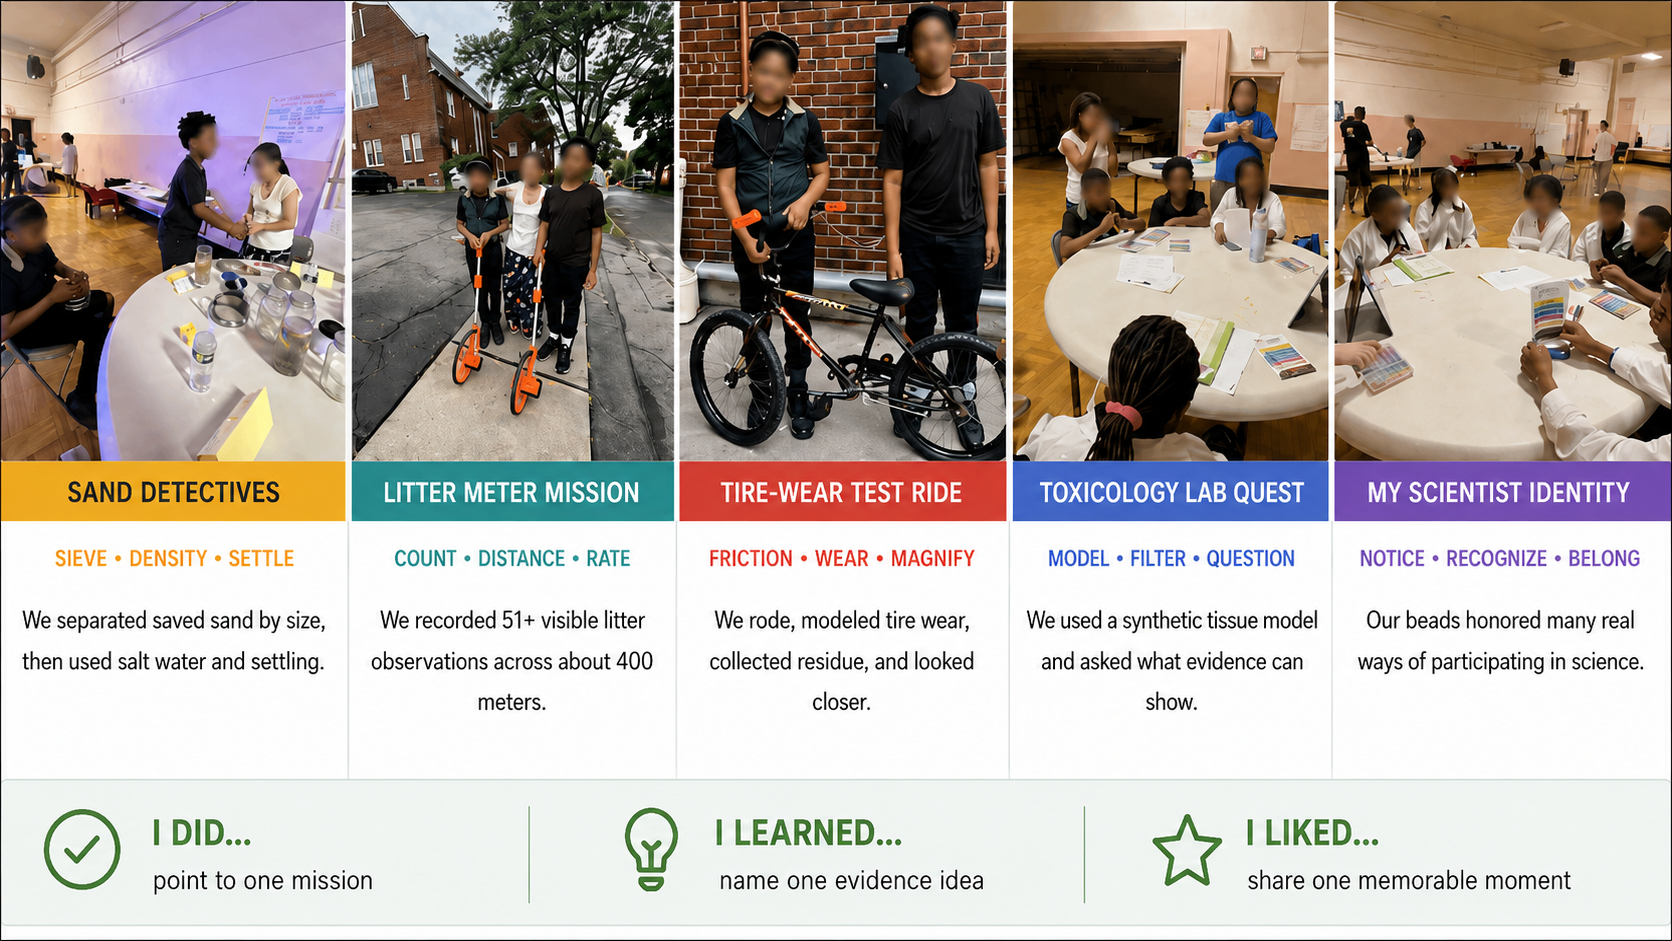
\includegraphics[
  width=0.96\textwidth,
  keepaspectratio
]{assets/artifact-previews/five_mission_learning_showcase.png}
\centering\scriptsize
{
\bfseries\color{DeepNavy}
Keep the Activity Present.\par
}
The camp recap kept the week's actual activities visible while youth reflected through \textit{I did}, \textit{I learned}, and \textit{I liked}. A learner could point, speak, or use the visual instead of recording a video. The memo is therefore one communication route, not the required route.\par
\end{minipage}
\hfill
\begin{minipage}[c]{0.49\textwidth}
{
\adaptationbox{A camera can create performance pressure or surveillance. Never infer private emotion from appearance, fluency, silence, or refusal. Do not post, send, or retain a memo beyond the agreed audience and purpose. Provide captioning, translation, AAC access, processing time, and a private or asynchronous option. Day 5 had photographs and a same-session transcript but no source video; this evidence system names that gap.}
}
\sourcebox{\scriptsize Video-memo archive \citep{campEvidence2026}; rich communicative environments \citep{downing2015classroom}; communication and behavior \citep{peckhamhardin2015behavior}; communicative competence \citep{jorgensen2018competence}.}
\end{minipage}
\end{center}

\endinput